\documentclass[svgnames,fragile]{beamer}

%\documentclass[a4paper]{article}

%% Language and font encodings
\usepackage[english]{babel}
\usepackage[utf8]{inputenc}
\usepackage[T1]{fontenc}
\usepackage{helvet}
\renewcommand{\familydefault}{\sfdefault}

% Bibliography
\usepackage[style=ieee,backend=biber,citestyle=numeric-comp,sorting=nty,doi=false,url=false,isbn=false]{biblatex}
\addbibresource{references.bib}
%% STOP BIBLATEX-BEAMER ERROR (start) %%
\usepackage{silence}
\WarningFilter{biblatex}{Patching footnotes failed}
%% STOP BIBLATEX-BEAMER ERROR (end) %%
\usepackage[utf8]{inputenc}
\usepackage[T1]{fontenc}

%% Sets page size and margins
\fontsize{11pt}{13pt}

%% Useful packages
\usepackage{amsmath}
\usepackage{xfrac}
\usepackage{graphicx}
\usepackage[colorinlistoftodos]{todonotes}
%\usepackage[colorlinks=true, allcolors=blue]{hyperref}
%\usepackage{titling}
\usepackage{parskip} %removes indents on new paragraphs
\usepackage[toc,page]{appendix}
\usepackage{chngpage}
\usepackage{graphicx} % graphics import
\usepackage{siunitx} % easy SI units
\usepackage{csquotes}
\usepackage{rotating}

%Figures
\usepackage{wrapfig}
\usepackage{caption}
\usepackage{subcaption}
\usepackage{chngpage}
\usepackage{float}

% Clever referencing
\usepackage[noabbrev]{cleveref}

% Change paragraph indentation
\setlength{\parskip}{10pt}
\setlength{\parindent}{0pt}

%figures to end
%\usepackage[nomarkers,nolists]{endfloat}
%\renewcommand{\efloatseparator}{\mbox{}}

%Colours for notes and shit
\usepackage[colorinlistoftodos]{todonotes}
\usepackage{xcolor}

\captionsetup{justification=centering}

\usepackage{xparse}

\newcommand{\diff}[3][]{\IfNoValueTF{#1}
{ \frac{\mathrm{d}{#2}}{\mathrm{d}{#3}} }
{ \frac{\mathrm{d}^{#1}{#2}}{\mathrm{d} {#3}^{#1} }} }

\newcommand{\pdiff}[3][]{\IfNoValueTF{#1}
{ \frac{\partial{#2}}{\partial{#3}} }
{ \frac{\partial^{#1} {#2}}{\partial {#3}^{#1}} } }

\newcommand{\fun}[3][]{\IfNoValueTF{#1}
{ \mathrm{#2}\mathopen{}\left(#3\right)\mathclose{} }
{ \mathrm{#2}^{#1}\mathopen{}\left(#3\right)\mathclose{} }}

\newcommand{\pdiffdiff}[3]{\frac{\partial^2{#1}}{\partial{#2}\partial{#3}}}

\renewcommand{\vec}[1]{\boldsymbol{#1}}

\newcommand{\Idx}{\;\mathrm{d}x}
\newcommand{\Real}{\mathbb{R}}
\newcommand{\Complex}{\mathbb{C}}
\newcommand{\Rational}{\mathbb{Q}}
\newcommand{\Integer}{\mathbb{Z}}
\newcommand{\Natural}{\mathbb{N}}


%\setbeamerfont{footnote}{size=\scriptsize}
\setbeamerfont{footnote}{size=\tiny}

\subtitle{}
\institute[]{Department of Engineering Mathematics\\ University of Bristol}

\usetheme{AnnArbor}
\usecolortheme{beaver}
\setbeamercolor{frametitle}{bg=gray!15!white,fg=darkred}
\setbeamercolor*{titlelike}{parent=palette primary}

\author{James Roff}

\date{}
\title[Instabilities of Pilot-Operated PRVs]{Modelling the Instabilities of a Pilot-Operated Pressure Relief Valve}

\begin{document}

\frame{\titlepage}

\begin{frame}{Introduction}
\begin{itemize}
    \item<1-> Pressure relief valves (PRVs) are an important safety feature for pressurised system
    \item<2-> The simplest PRV is a spring-operated pressure relief valve
    \item<3-> A more complex design is a pilot-operated PRV which uses the tank pressure to hold the valve closed
    \item<4-> However, both designs can suffer from instabilities
    \item<5-> One very damaging instability is a chatter instability, with high frequency oscillations causing impacts
\end{itemize}
\end{frame}

\begin{frame}{Existing Research}
\begin{itemize}[noitemsep]
%\itemsep0em
    \item<1-> Unstable operation has been a known phenomena since the 1960s \footfullcite{Kasai1968OnSystem}
    \item<2-> The cause of chatter instability for spring-operated PRVs has been identified as an acoustic quarter-wave interaction \footfullcite{Hos2017DynamicRecommendations}
    \item<3-> Only very simple models exist for pilot-operated PRVs \footfullcite{Ye2009DynamicSystem}
    \item<4-> A chatter like instability has recently been observed in pilot-operated PRVs \footfullcite{Allison2015TestingValves}
\end{itemize}
\end{frame}

\begin{frame}{Pilot-Operated PRV Schematic}
\centering
\begin{minipage}{0.8\textwidth}
    \begin{figure}[ht]
    % COMPLETE DIAGRAM
    \begin{subfigure}{0.6\textwidth}
    \centering
    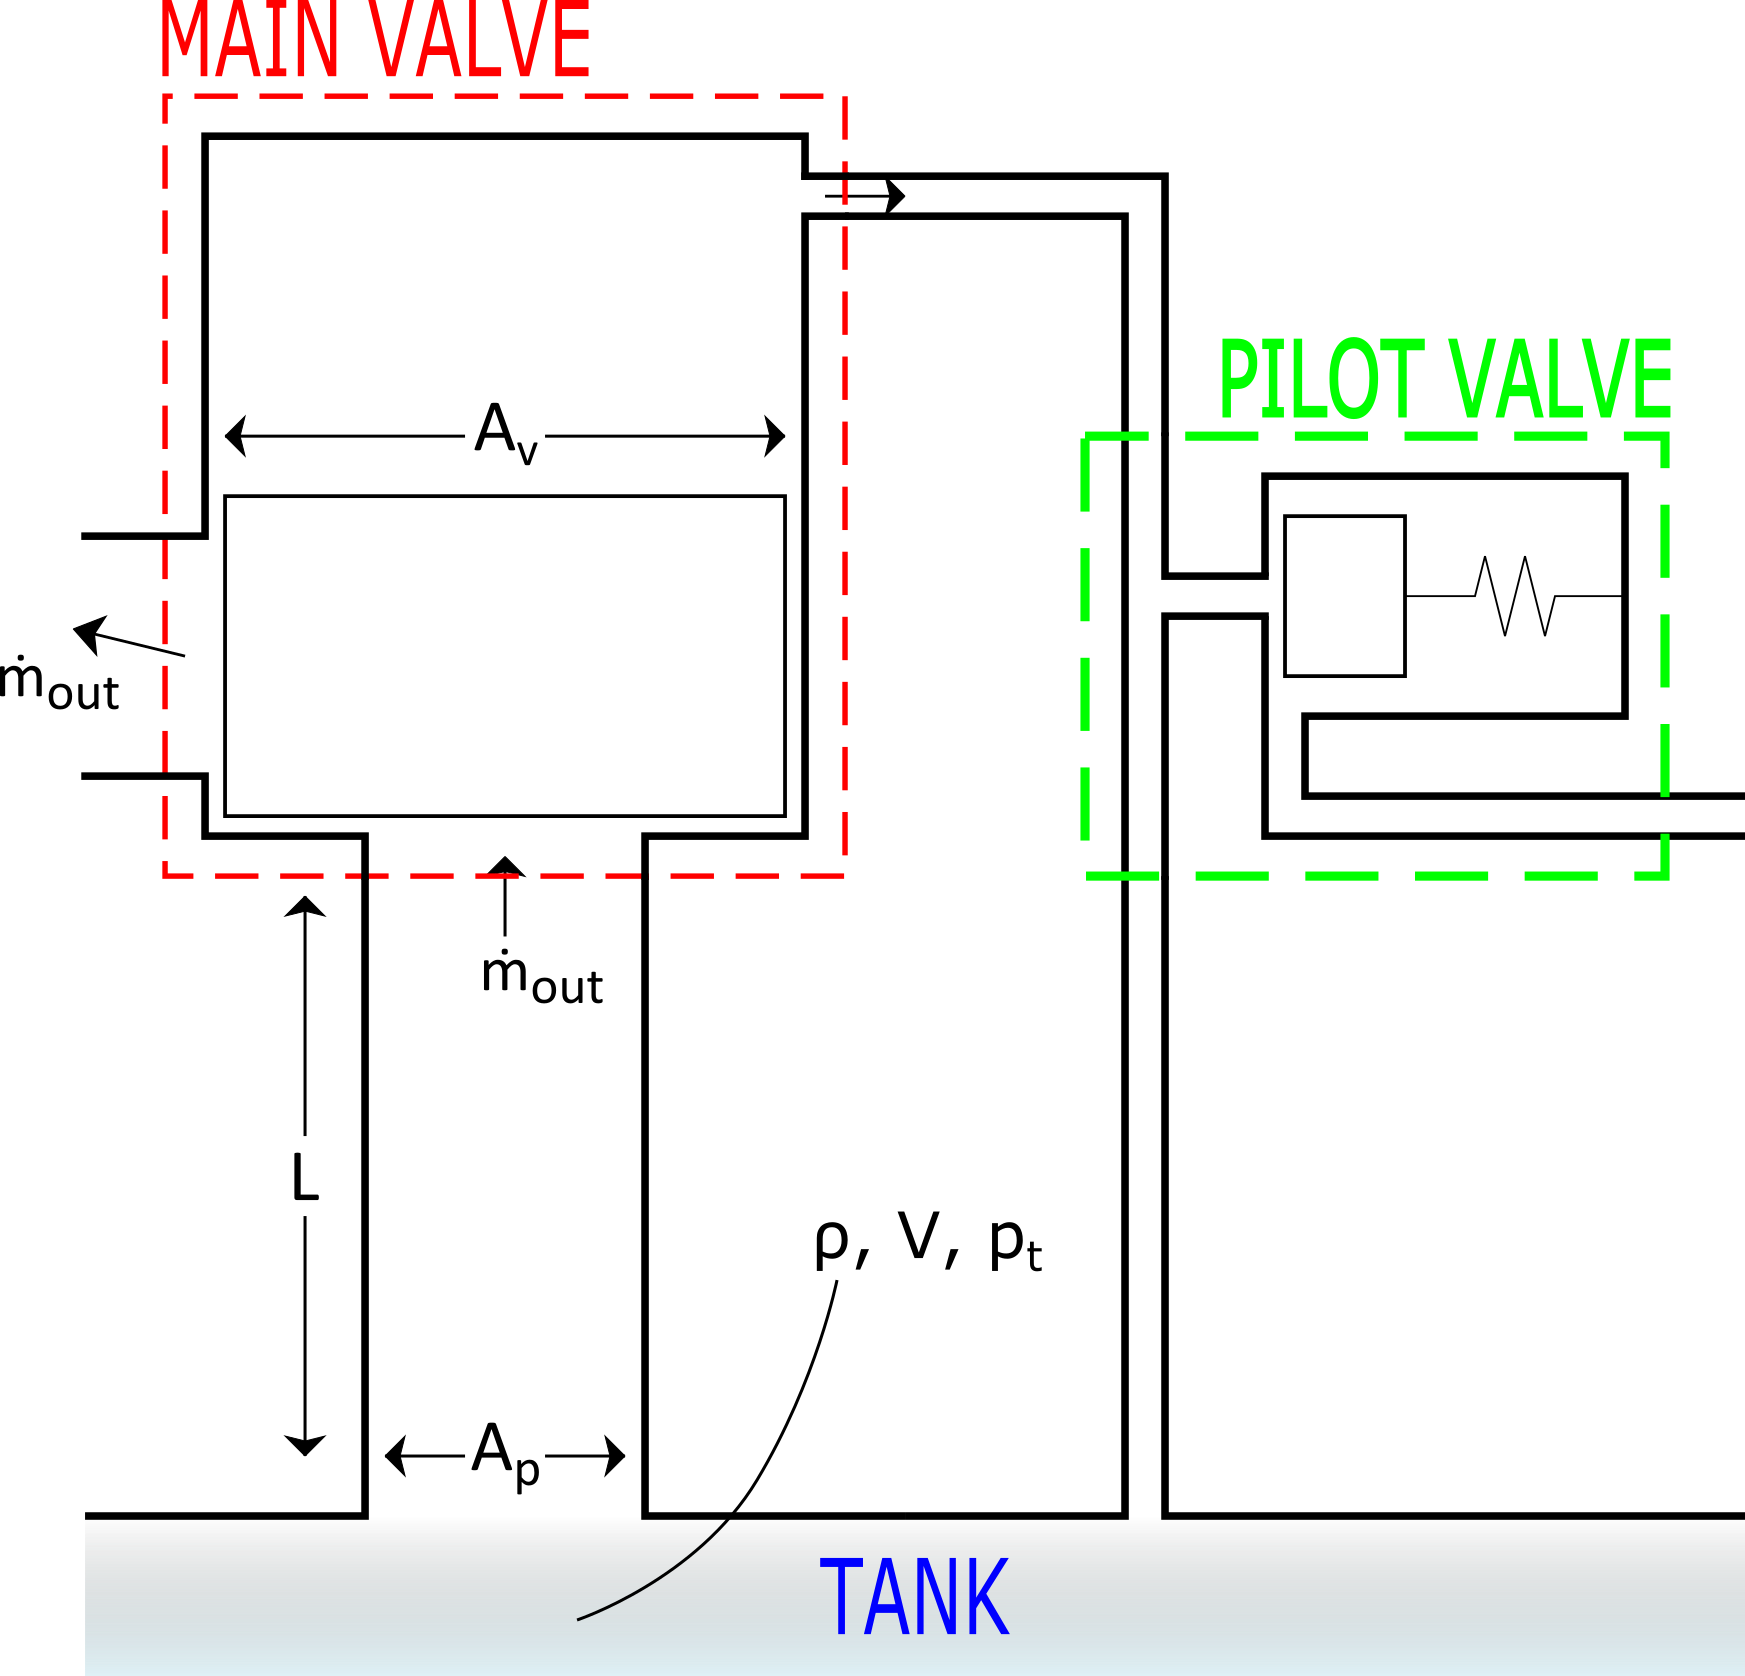
\includegraphics[width=\textwidth]{Diagrams/Diagram.png}
    \caption{Complete valve}
    \label{fig: DiagramComp}
    \end{subfigure}
    \hfill
    % Separate valve figures
    \begin{minipage}{0.3\textwidth}
        % MAIN DIAGRAM
        \begin{subfigure}{\textwidth}
        \centering
        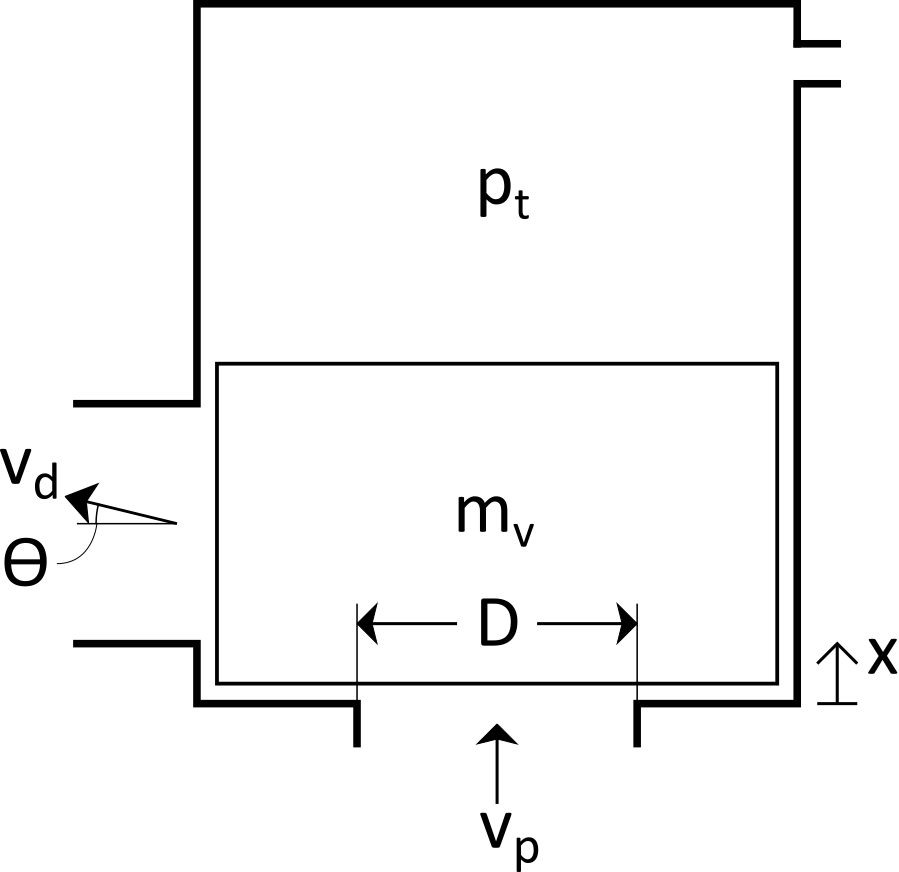
\includegraphics[width=\textwidth]{Diagrams/Diagram-Main.png}
        \caption{Main Valve}
        \label{fig: DiagramMain}
        \end{subfigure}
        % PILOT DIAGRAM
        \begin{subfigure}{\textwidth}
        \centering
        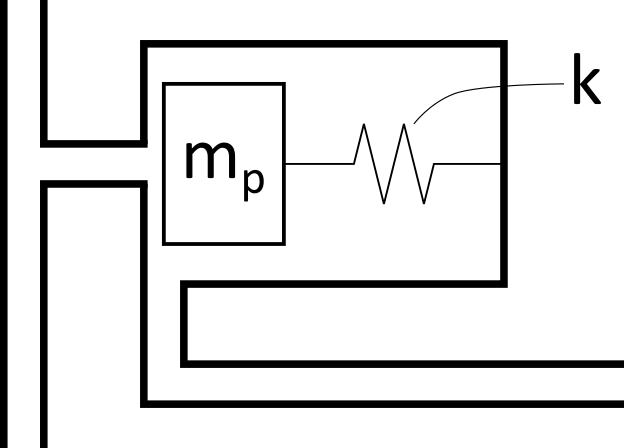
\includegraphics[width=\textwidth]{Diagrams/Diagram-Pilot.png}
        \caption{Pilot Valve}
        \label{fig: DiagramPilot}
        \end{subfigure}
    \end{minipage}
    % Figure caption and label
    \caption{Diagram of pilot-operated pressure relief valve}
    \label{fig: Diagram}
\end{figure}
\end{minipage}
\end{frame}

\begin{frame}{Valve-closing model - Valve}
\begin{itemize}
    \item<1-> Initially neglected the inlet piping
    \item<2-> Consider the valve closing so pilot valve does not need to be considered
    \item<3-> Three forces acting on the valve:
    \begin{itemize}
        \item<4-> Tank pressure
        \item<5-> Dome pressure
        \item<6-> Fluid momentum
    \end{itemize}
    \item<7-> Equation of motion is:
    \begin{equation*}
        m_v \ddot{x} + c_v \dot{x} = - A_p p_t + A_p p_d + \dot{m}_{out} v_p
    \end{equation*}
\end{itemize}
\end{frame}

\begin{frame}{Valve-closing model - Tank}
\begin{itemize}
    \item<1-> Consider a constant mass flow into the tank, $\dot{m}_{in}$
    \item<2->
    \item<3-> The pressure inside the tank is given by:
    \begin{equation*}
        \dot{p}_t = \frac{a^2}{V} \left( \dot{m}_{in} - \dot{m}_{out} \right)
    \end{equation*}
\end{itemize}
\end{frame}

\begin{frame}{Valve-closing model - Non-dimensionalisation}
\begin{itemize}
    \item<1-> Equations of motion can be non-dimensionised using reference distance, pressure and time
    \begin{equation*}
        x_{ref} = \frac{1}{C_d} \sqrt{\frac{A_v - A_p}{4 \pi}} \, , \quad
        p_{ref} = \frac{\dot{m}_{in}\,^2}{2 A_p \left( A_v - A_p \right)} \, , \quad
        t_{ref} = \frac{m_v}{c_v}
    \end{equation*}
    \item<2-> The dimensionless equations are
    \begin{equation}
    \begin{split}
        \tilde{x}'' + \tilde{x}' &= \alpha \tilde{p} \left( \tilde{x}^2 - 1 \right) \\
        \tilde{p}' &= \beta \left( 1 - \tilde{x} \sqrt{\tilde{p}} \right)
    \end{split}
    \end{equation}
\end{itemize}
\end{frame}

\begin{frame}{Stability Analysis}
\begin{itemize}
    \item<1-> One equilibrium of interest at $\tilde{x} = 1$ and $\tilde{p} = 1$
    \item<2-> Stability analysis reveals
    \begin{itemize}
        \item<3-> Two negative eigenvalues of
        \begin{equation*}
            \lambda_1 = - \frac{1}{2} \beta \qquad
            \lambda_2 = - \frac{1}{2} - \sqrt{2 \alpha + \frac{1}{4}}
        \end{equation*}
        \item<4-> One positive eigenvalue of
        \begin{equation*}
            \lambda_3 = - \frac{1}{2} + \sqrt{2 \alpha + \frac{1}{4}}
        \end{equation*}
    \end{itemize}
    %\item<5-> Hence, valve open equilibrium is a saddle
\end{itemize}
\end{frame}

\begin{frame}{Simulation Results}
\begin{figure}
    \centering
    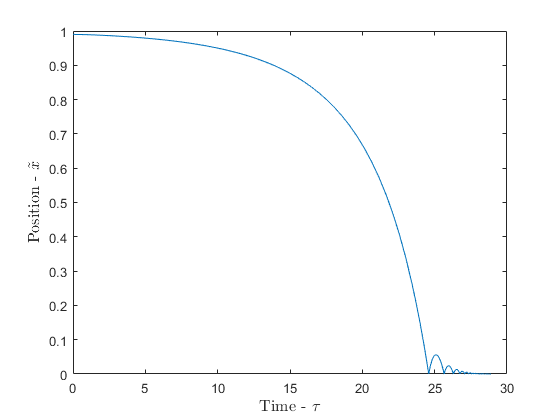
\includegraphics[width=0.7\textwidth]{Figures/Example/PositionTimeTrajectory.png}
    \caption{Time trajectory of valve position}
\end{figure}
\end{frame}

\begin{frame}{Low-flow rates}
\begin{itemize}
    \item<1-> While the valve is closing, only low mass inflows will occur
    \item<2-> Consider the limit that $\dot{m}_{in} \rightarrow 0$, so
    \begin{itemize}
        \item<3-> $\alpha \rightarrow 0$
        \item<4-> $\beta \rightarrow \infty$
    \end{itemize}
    \item<5-> The unstable eigenvalue $\lambda_3 \rightarrow 0$
    \item<6-> A family of equilibrium exist where $1 - x \sqrt{p} = 0$
\end{itemize}
\end{frame}

\begin{frame}{Phase-Portrait}
\begin{figure}
    \centering
    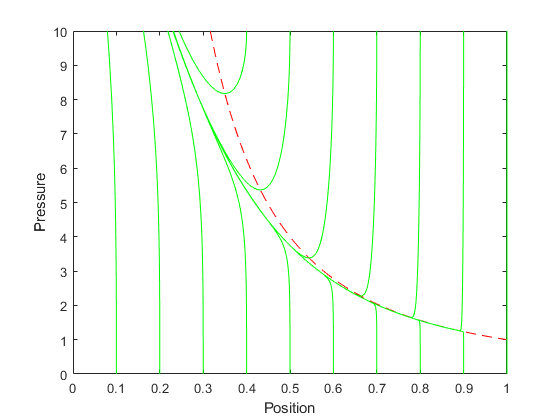
\includegraphics[width=0.7\textwidth]{Figures/LowFlow/LargePhasePortrait-b=10.png}
    \caption{Phase-portrait for $\alpha = 0.01$ and $\beta = 10$}
\end{figure}
\end{frame}

\begin{frame}{Valve Closing with Inlet Piping - Fluid}
\begin{itemize}
    \item<1-> Fluid in the piping is slightly compressible, which must fulfil
    \begin{equation*}
    \begin{split}
        \pdiff{p}{t} + v \pdiff{p}{\eta} + \rho a^2 \pdiff{v}{\eta} &= 0 \\
        \pdiff{v}{t} + v \pdiff{v}{\eta} + \frac{1}{\rho} \pdiff{p}{\eta} &= \lambda \frac{L}{D} v \left| v \right|
    \end{split}
    \end{equation*}
    \item<2-> The pressure and velocity distributions in the pipe are given by
    \begin{equation*}
    \begin{split}
        p(\eta,t) &= p_t(t) + B(t) \fun{sin}{2\pi \frac{\eta}{4L}} \, ,\\
        v(\eta,t) &= v_L(t) + C(t) \fun{cos}{2\pi \frac{\eta}{4L}} \, .
    \end{split}
    \end{equation*}
    \item<3-> A collocation method ensures the PDE is satisfied at $\eta = \frac{L}{2}$
\end{itemize}
\end{frame}

\begin{frame}{Valve Closing with Inlet Piping - Full equations}
Including the quarter-wave gives:
\begin{equation*}
\begin{split}
    \ddot{x} &= - \frac{c_v}{m_v} \dot{x} + \frac{A_v}{m_v} B + \frac{\zeta^2}{m_v A_p} x^2 B + \frac{\zeta^2}{m_v A_p} x^2 p_t \\
    \dot{p}_t &= \frac{a^2}{V} \left( \dot{m}_{in} - \rho A_p C(t) - \sqrt{2} \pi D C_d x(t) \sqrt{\rho} \sqrt{p_t(t) + B(t)} \right) \, , \\
    \dot{B} &= a^2 \rho \frac{\pi}{2L} C - \sqrt{2} \dot{p}_t - \frac{\pi}{2L} \frac{\sqrt{2} \pi D C_d}{A_p \sqrt{\rho}} x B \sqrt{p_t + B} - \frac{\pi \sqrt{2}}{4L} B C \, , \\
    ~
    \dot{C} &=
    \frac{\pi \zeta}{2 A_p L \sqrt{\rho}} x C \sqrt{p_t + B}
    + \frac{\pi \sqrt{2}}{4L} C^2
    - \frac{\pi}{2 L \rho} B
    - \frac{\sqrt{2} \zeta}{A_p \sqrt{\rho}} v \sqrt{p_t + B} \\ &\quad %linebreak
    + \frac{2 - \sqrt{2}}{2} \frac{\zeta}{A_p \sqrt{\rho}} \frac{x}{\sqrt{p_t + B}} \dot{p}_t 
    - \frac{\sqrt{2}\pi\zeta a^2 \rho}{4 L A_p \sqrt{\rho}} \frac{x C}{\sqrt{p_t + B}}
    + \frac{\sqrt{2}\pi\zeta^2}{4L A_p\,^2 \rho} x^2 B \\ &\quad %linebreak
    + \frac{\pi \zeta}{4 L A_p \sqrt{\rho}} \frac{x B C}{\sqrt{p_t + B}}
    + \lambda \frac{\sqrt{2}L}{4 D} \left( \sqrt{2} v_L + C \right) \left| \sqrt{2} v_L + C \right|
\end{split}
\end{equation*}
\end{frame}

% \begin{frame}{Valve Closing with Inlet Piping - Quarter wave}
% Blank frame
% \end{frame}

\begin{frame}{Next steps}
\begin{itemize}
    \item<1-> Analyse the full valve closing model
    \begin{itemize}
        \item<2-> Non-dimensionalise the equations
        \item<3-> Stability analysis along unstable manifold
        \item<4-> Find Hopf bifurcation corresponding to Chatter
    \end{itemize}
    \item<5-> Include the pilot valve dynamics
    % \begin{itemize}
    %     \item Allows modelling of 
    % \end{itemize}
    \item<6-> Include variation in dome pressure
\end{itemize}
\end{frame}

\end{document}